%% ---------------------------------------------------------------------------
%% resultados.tex
%%
%% Capítulo 4: Descripción del trabajo realizado
%% Estructura según los Lineamientos para los Trabajos Finales de Graduación
%% V4.1, CE-5601 (Opción 1): 4.1 Descripción del proceso de solución y
%% 4.2 Análisis de los resultados obtenidos.
%%
%% Fuente de todas las cifras: scripts/rl/CONTEXTO.md y realtime/ESTADO_APP_ANDROID.md
%% de la rama SLAM_RealTime (commit 83ff88d, 16/10/2026). Los comentarios
%% "% CTX §x" indican la sección de CONTEXTO.md de donde sale cada dato.
%% Las cifras de la Sección 4.2 son preliminares (código del 7 al 12/10/2026)
%% hasta la corrida final con el código congelado. Origen por tabla:
%%   tab:res-campo: sesiones en vivo (CTX §4.21); tab:res-gps-degradado: banco
%%   sobre los cuadros en vivo (§4.22-4.23); tab:res-filtro y 14:05/14:18 de
%%   tab:res-solo-visual: corridas de §4.17 (código del 7/10; a 30 s reproducidas
%%   con el del 12/10, §4.27); resto de tab:res-solo-visual: §4.25; RL: §4.31-4.33.
%%
%% Convención de escritura: una oración por línea del archivo fuente.
%% ---------------------------------------------------------------------------

\chapter{Descripción del trabajo realizado}
\label{ch:resultados}

Este capítulo describe el trabajo realizado para alcanzar los objetivos del proyecto, siguiendo el marco metodológico del Capítulo~\ref{ch:solucion}.
La Sección~\ref{sec:res-proceso} detalla el proceso de solución: los requerimientos de la plataforma, su arquitectura, las decisiones de diseño tomadas en cada incremento y el mecanismo de aprendizaje por refuerzo.
La Sección~\ref{sec:res-analisis} analiza los resultados obtenidos frente a cada objetivo específico, en cuanto al comportamiento en tiempo real, la precisión de la localización y el aporte del aprendizaje por refuerzo, y cierra con las limitaciones de la solución.
Como no se dispone de una trayectoria de referencia de alta precisión para las grabaciones propias, cada magnitud se contrasta con la medición independiente más confiable del teléfono: la posición con el GPS, la rotación con el giroscopio y la rapidez con la velocidad Doppler (Sección~\ref{sec:met-fase3}).

% ===========================================================================
\section{Descripción del proceso de solución}
\label{sec:res-proceso}
% ===========================================================================

Esta sección sigue los incrementos de la Fig.~\ref{fig:met-proceso}.
Primero se presentan los requerimientos obtenidos en la Fase~1 y la arquitectura resultante de la Fase~2.
Después se describen las decisiones de diseño de cada incremento, cada una con el problema que la motivó, las alternativas consideradas y la medición que permitió elegir entre ellas.

% ---------------------------------------------------------------------------
\subsection{Requerimientos de la plataforma}
\label{sec:res-requerimientos}
% OE1. CTX §1, §4.7, §4.9, §4.20; ESTADO_APP_ANDROID §4, §5, §6.

Los requerimientos se derivaron de los objetivos del proyecto y de las características medidas del dispositivo, ya que varias de ellas difieren de los valores nominales.
La cámara del Samsung Galaxy S23 entrega 1280$\times$720 píxeles a 30 cuadros por segundo, con los parámetros intrínsecos de su calibración de fábrica, que el teléfono envía al conectarse, y una distorsión no corregida de hasta 17~px en las esquinas.
Cada cuadro tarda de 60 a 75~ms en llegar a la aplicación y, por cable, de 66 a 70~ms en llegar a la computadora en la mediana y de 73 a 76~ms en el percentil 95, de modo que una parte importante de la latencia ocurre antes del procesamiento.
El GPS, que la aplicación obtiene del proveedor de ubicación fusionado de Android, entrega una solución por segundo en el vehículo, con su velocidad Doppler y una antigüedad mediana de 0,4 a 0,5~s, y el giroscopio y el acelerómetro entregan unas 53 muestras por segundo.
Todas las fuentes comparten el reloj de arranque del teléfono, que es el que se usa para alinearlas, mientras que su hora Unix difiere de la de la computadora en una cantidad que cambia de un día a otro.

La Tabla~\ref{tab:res-requerimientos} presenta los requerimientos resultantes, agrupados en funcionales, computacionales y temporales, junto con la forma de verificar cada uno.
Los valores de RT-1 y RT-2 son los que se emplearon como referencia durante el desarrollo; su validación por parte del profesor asesor, junto con los criterios cuantitativos de los demás requerimientos, se encuentra pendiente.

Las métricas de las Secciones~\ref{sec:tiempo-real} y~\ref{sec:metricas} se implementaron en dos lugares.
El canal de procesamiento registra por cuadro el tiempo de cada etapa, la latencia, el descarte y la frecuencia efectiva.
Una herramienta de evaluación calcula sobre cada sesión el error de trayectoria con alineación rígida, la deriva desde un inicio común y durante cortes simulados del GPS, la escala frente a la Doppler y la rotación frente al giroscopio.
El error relativo de pose y la utilización de recursos computacionales todavía no forman parte de esa herramienta.

% Pendiente para discutir con la contraparte: Actualizar la tabla con los valores validados por el asesor e indicar en qué equipo se exigen los requerimientos temporales.

\begin{table}[H]
\centering
\caption{Requerimientos propuestos para la plataforma}
\label{tab:res-requerimientos}
\footnotesize
\begin{tabularx}{\textwidth}{@{}>{\raggedright\arraybackslash}p{1.1cm}>{\raggedright\arraybackslash}X>{\raggedright\arraybackslash}p{4.6cm}@{}}
\toprule
\textbf{Id.} & \textbf{Requerimiento} & \textbf{Verificación} \\
\midrule
RF-1 & Recibir en vivo del teléfono el video, las posiciones GPS con su velocidad Doppler y las mediciones inerciales, con marcas de tiempo de un reloj común. & Comparación de lo recibido con lo grabado por el teléfono. \\
RF-2 & Procesar grabaciones con el mismo canal y el mismo formato que en vivo, con un modo de ejecución determinista. & Repetición de corridas sobre una misma grabación. \\
RF-3 & Estimar en cada cuadro la posición y el rumbo en un plano métrico, combinando la cámara, el giroscopio y el GPS. & Predicción frente a cada solución GPS nueva. \\
RF-4 & Mantener la estimación durante las pérdidas del GPS y rechazar las soluciones incompatibles con la predicción. & Cortes simulados y GPS degradado de forma sintética. \\
RF-5 & Ejecutar una misma grabación en modo exclusivamente visual. & Comparación del cuarto objetivo. \\
RF-6 & Ajustar el peso de una fuente mediante una política con estado y recompensa explícitos. & Protocolo de evaluación del tercer objetivo. \\
RF-7 & Mostrar durante la operación el video, el estado del sistema y la trayectoria, y registrar cada sesión. & Sesiones en vivo y sobre grabaciones. \\
\addlinespace
RC-1 & Ejecutarse en una computadora con tarjeta gráfica NVIDIA y Linux, incluida una portátil a bordo del vehículo, sin depender de una conexión a internet. & Prueba con la red desconectada y prueba de campo. \\
RC-2 & Mantener el costo de la fusión y de la política despreciable frente al presupuesto de cada cuadro. & Tiempo por etapa. \\
\addlinespace
RT-1 & Latencia de la captura al resultado con percentil 95 menor que 150~ms. & Latencia medida con el reloj del teléfono. \\
RT-2 & Frecuencia efectiva de al menos 10~Hz. & Ecuación~\eqref{eq:descarte}. \\
RT-3 & Latencia acotada ante sobrecarga, mediante el descarte de cuadros. & Cola de una posición (Fig.~\ref{fig:descarte}). \\
\bottomrule
\end{tabularx}
\end{table}

% ---------------------------------------------------------------------------
\subsection{Arquitectura de la plataforma}
\label{sec:res-arquitectura}
% OE2. CTX §2 (decisiones 1-4), §4.1, §4.2, §4.4, §4.9, §4.19, §4.20, §4.24;
% ESTADO_APP_ANDROID §3, §4.
%
% Para el documento de arquitectura (apéndice), módulos de realtime/:
%   sources (fuentes intercambiables, protocolo, almacenamiento causal, reloj del
%   teléfono); pipeline (hilos, cola, odometría visual, hilo de profundidad, fusión,
%   métricas); depth_scale (rapidez y compuerta de detenido); fusion (EKF, giroscopio,
%   validación, modo solo visual); session/run_live/run_replay (sesiones y registro);
%   live_window (interfaz); cache; evaluate; phone_simulator; rl/env y rl/policy.

La Fig.~\ref{fig:res-arquitectura} muestra la arquitectura de la plataforma.
Se compone de dos programas independientes, la aplicación del teléfono y el canal de procesamiento de la computadora, unidos únicamente por el protocolo de red.

\begin{figure}[H]
\centering
\begin{tikzpicture}[
  font=\scriptsize,
  caja/.style={draw, rounded corners=2pt, align=center, fill=white, inner sep=2pt, minimum height=8mm},
  grupo/.style={draw, thick, rounded corners=3pt, fill=black!4, inner sep=2.5mm},
  flecha/.style={-{Stealth[length=1.7mm]}, thick},
  doble/.style={{Stealth[length=1.7mm]}-{Stealth[length=1.7mm]}, thick},
  rotulo/.style={font=\scriptsize, align=center}
]
% --- teléfono ---
\node[caja, text width=19mm] (cam) at (1.3,2.6)  {Cámara\\30 cuadros/s};
\node[caja, text width=19mm] (gps) at (1.3,1.0)  {GPS\\posición y Doppler};
\node[caja, text width=19mm] (imu) at (1.3,-0.6) {IMU\\53 muestras/s};
\node[caja, text width=19mm] (rec) at (1.3,-2.2) {Grabación local\\(opcional)};
\node[anchor=south, font=\footnotesize\bfseries, align=center] (tt) at (1.3,3.25) {Teléfono\\(aplicación)};
\begin{scope}[on background layer]
  \node[grupo, fit=(tt)(cam)(rec)] (tel) {};
\end{scope}
% --- computadora ---
\node[caja, text width=18mm] (cap) at (5.9,2.6)  {Hilo de captura};
\node[caja, text width=15mm] (cola) at (8.15,2.6) {Cola de una posición};
\node[caja, text width=25mm] (vo)  at (10.75,2.6) {Odometría visual\\ORB, RANSAC y pose};
\node[caja, text width=27mm] (dep) at (10.75,1.0) {Hilo de profundidad\\(rapidez, $\approx$3~Hz)};
\node[caja, text width=21mm] (sen) at (6.05,-0.6) {Hilo de GPS e IMU\\almacenamiento causal};
\node[caja, text width=20mm, fill=black!12] (ekf) at (14.0,1.0) {Filtro de Kalman extendido};
\node[caja, text width=12mm, dashed] (pol) at (14.65,-0.6) {Política\\tabla $Q$};
\node[caja, text width=22mm] (win) at (7.6,-2.4) {Ventana: video, estado y mapa};
\node[caja, text width=22mm] (log) at (10.75,-2.4) {Registro de la sesión y caché};
\node[caja, text width=20mm] (eva) at (14.0,-2.4) {Evaluación fuera de línea};
\node[anchor=south, font=\footnotesize\bfseries, align=center] (tc) at (10.0,3.25) {Computadora (canal de procesamiento)\\{\scriptsize\mdseries fuente: teléfono en vivo, grabación o simulador}};
\begin{scope}[on background layer]
  \node[grupo, fit=(tc)(cap)(sen)(ekf)(pol)(eva)(win)] (pc) {};
\end{scope}
% --- protocolo ---
\draw[flecha] (cam.east) -- node[rotulo, above] {TCP 5000} node[rotulo, below] {video} (cap.west);
\draw[thick] (gps.east) -- ++(0.3,0) |- (imu.east);
\draw[doble] ([xshift=3mm]imu.east) -- node[rotulo, above] {UDP 5001} node[rotulo, below] {GPS, IMU,\\estado, hora} (sen.west);
% --- flujo interno ---
\draw[flecha] (cap) -- (cola);
\draw[flecha] (cola) -- (vo);
\draw[flecha] (vo) -- node[rotulo, right] {características} (dep);
\draw[flecha] (vo.east) -| node[rotulo, pos=0.3, above] {giro de respaldo} (ekf.north);
\draw[flecha] (dep) -- node[rotulo, above] {$v^{\mathrm{cam}}$} (ekf);
\draw[flecha] (sen.east) -- node[rotulo, above] {posición, Doppler y giro $\Delta\psi$} (12.45,-0.6) |- ([yshift=-2.5mm]ekf.west);
\draw[flecha, dashed] (pol.north) -- node[rotulo, right] {$\lambda$} (pol.north |- ekf.south);
\draw[thick] ([xshift=2mm]ekf.south west) -- ([xshift=2mm]ekf.south west |- 0,-1.55) -- node[rotulo, above, pos=0.6] {estado por cuadro} (7.6,-1.55);
\draw[flecha] (7.6,-1.55) -- (win.north);
\draw[flecha] (10.75,-1.55) -- (log.north);
\draw[flecha] (log) -- (eva);
\end{tikzpicture}
\caption[Arquitectura de la plataforma]{Arquitectura de la plataforma. La aplicación y el canal de procesamiento solo comparten el protocolo de red. La política, en línea discontinua, aún no está integrada en el canal. Fuente: elaboración propia.}
\label{fig:res-arquitectura}
\end{figure}

\textbf{Aplicación y protocolo.}
La aplicación actúa como servidor.
Al conectarse, la computadora recibe por TCP los parámetros de la cámara y después cada cuadro en formato JPEG con su instante de captura, y por UDP cada posición GPS y cada muestra de la IMU, con el mismo formato con que el teléfono las guarda en sus archivos.
Por el mismo canal UDP, la computadora inicia o detiene la grabación en el teléfono y consulta su hora.
El teléfono no encola cuadros: si la red está ocupada los descarta, de modo que el retraso no crece.

\textbf{Canal de procesamiento.}
El canal separa en hilos distintos la captura, la recepción de los sensores y el procesamiento.
Los cuadros llegan a una cola de una sola posición que descarta el más antiguo (Sección~\ref{sec:tiempo-real}), y las posiciones y muestras inerciales se almacenan de forma causal, de modo que cada cuadro solo accede a lo recibido hasta su marca de tiempo.
El hilo de procesamiento ejecuta la odometría visual y una etapa del filtro por cuadro, mientras que la rapidez del modelo de profundidad se calcula en un hilo aparte que reutiliza las características de la odometría visual.
Cada sesión se guarda en disco, con el estado del filtro por cuadro, las posiciones, las muestras inerciales y las métricas temporales, y se muestra durante la operación en una ventana con el video y el mapa de la trayectoria fusionada.
Como la diferencia entre el reloj del teléfono y el de la computadora varió de un día a otro entre $-56$ y $+132$~ms, la latencia desde la captura se mide consultando la hora del teléfono cada 0,5~s y tomando la consulta de ida y vuelta más rápida del último minuto; por cable, el error de esta sincronización fue de a lo sumo 0,5~ms.

\textbf{Modos de ejecución.}
Las fuentes son intercambiables: el teléfono en vivo, una grabación o un simulador del teléfono, que sirve una grabación con el protocolo de la aplicación y permitió integrar el canal y la interfaz antes de usar el teléfono.
Sobre grabaciones, el modo determinista produjo resultados idénticos bit a bit en corridas repetidas y, en la computadora de escritorio, predijo el descarte y la latencia del modo estricto con diferencias cercanas a 1~ms.
Sus resultados se guardan en una caché indexada por el contenido de la grabación, las opciones de la corrida y el código que la produce, de modo que un cambio en la grabación, en las opciones o en los módulos del canal obliga a reprocesar.
El modo exclusivamente visual ejecuta la misma grabación sin usar el GPS después del arranque y es la línea base del cuarto objetivo.
El detalle de los módulos y del protocolo corresponde al documento de arquitectura, entregable del segundo objetivo.

% Pendiente para discutir con la contraparte: Incluir el documento de arquitectura (módulos, interfaces y protocolo) como apéndice y referenciarlo aquí.

% ---------------------------------------------------------------------------
\subsection{Estimación de la escala métrica}
\label{sec:res-escala}
% OE2. CTX §3.1, §3.2, §3.3, §4.3, §4.12, §4.13, §4.15.
% No se usan las tablas de trayectorias de §3.3 (24,64 -> 16,89 m y ATE en KITTI):
% CONTEXTO las marca "a verificar" porque salieron del encadenamiento de poses viejo.

El análisis del punto de partida mostró que la plataforma previa no disponía de una escala propia para la cámara.
La recuperación de la pose entrega una traslación de norma unitaria (Sección~\ref{sec:escala}), y la plataforma previa le asignaba en cada paso la longitud medida por el GPS y orientaba la trayectoria hacia la dirección del GPS, de modo que no existían dos fuentes independientes que fusionar.
Una medición con el GPS degradado de forma sintética lo confirmó: el error de la odometría visual aumentó de 41 a 250~m cuando la desviación estándar del ruido añadido pasó de 3 a 10~m, algo que no ocurriría con una estimación visual independiente.

Se evaluaron tres fuentes de escala: la derivada de las posiciones GPS, la recuperación por plano de tierra y la profundidad estimada por un modelo monocular.
En KITTI, con la trayectoria de referencia empleada solo para evaluar, el error mediano de escala fue cercano a 45~\% con el GPS a 1~Hz y a 50~\% con una implementación simple del plano de tierra, por lo que se eligió el modelo Depth Anything~V2 en su variante métrica para exteriores \cite{yang2024depthanything}, que además no consume el GPS.

El primer intento de integrarlo falló por la base de triangulación y no por el modelo.
A 30 cuadros por segundo el vehículo avanza unos 0,14~m entre cuadros consecutivos, lo que no basta para triangular puntos a 10--50~m: con esa separación, la razón entre la escala estimada y la real fue de 2,64, mientras que entre cuadros separados 0,33~s, con una base de 2,38~m, fue de 1,08.
Por ello la Ecuación~\eqref{eq:escala-metrica} se evalúa entre cuadros separados 0,33~s, solo con puntos de entre 3 y 60~m de profundidad, y su resultado se suaviza con la mediana de las últimas siete estimaciones.
Sobre las siete secuencias utilizables de KITTI, el error mediano de escala osciló entre 10 y 37~\% en las seis urbanas y alcanzó 63~\% en la de autopista; es mínimo entre 6 y 12~m/s y crece por debajo de 6~m/s, hasta 57~\% bajo 2~m/s por falta de base, y por encima de 12~m/s, cuando la escena se aleja del rango útil del modelo.

En las grabaciones en vehículo apareció una dependencia adicional.
El modelo reescala cada imagen a un lado corto fijo sin conocer la distancia focal, de modo que recortar la franja inferior de la imagen, donde aparece el capó, cambiaba la escala de píxeles y reducía la profundidad estimada en cerca de 30~\%.
Por esa razón, en lugar de recortar la imagen se aplica una máscara que impide detectar características en esa franja, y el modelo recibe la imagen completa.
Aun así, con la máscara la distancia medida por la cámara superó a la del GPS en 10~\% en una grabación y en 59~\% en otra, lo que llevó a tratar la rapidez de la cámara como una medición cuyo factor de escala $\kappa$ estima el filtro con la Doppler (Ecuación~\eqref{eq:estado-ekf}), y no como una escala absoluta.
La estimación corre en su propio hilo, a unos 3~Hz; en la computadora de escritorio sumó 2,3~ms a la mediana de la latencia, sin reducir la frecuencia de 30~Hz, aunque cada inferencia del modelo tarda unos 88~ms.

\textbf{Detección del vehículo detenido.}
Con el vehículo detenido no hay base de triangulación, y la cámara reportaba una rapidez mediana de 0,44 a 0,64~m/s.
La razón entre inliers y correspondencias y el flujo de las características no separaron al vehículo detenido del que avanza lentamente: el capó oculta los puntos cercanos, el avance entre cuadros consecutivos es menor que un píxel y el teléfono gira en los altos por el cabeceo del vehículo.
Sí los separó el residuo que queda después de ajustar la rotación pura que mejor explica el movimiento de los puntos entre cuadros separados 0,33~s, ya que un giro sin avance no produce paralaje: su mediana fue de 1,1 a 1,3~px con el vehículo detenido, de 3,0~px a 1--1,5~m/s y de 7,6 a 8~px por encima de 5~m/s.
La regla adoptada declara la detención cuando el residuo es menor que 2~px en dos estimaciones seguidas y la rapidez estimada es menor que 3~m/s, y la retira cuando supera 3~px; el límite de rapidez evita falsas detenciones en autopista, donde la escena lejana también deja poco paralaje.
En las dos grabaciones completas del 30 de septiembre, la regla detectó el 85 y el 97~\% de los cuadros con el vehículo detenido según el GPS, marcó como detenidos solo el 1,1 y el 0,6~\% de los cuadros a más de 1~m/s, y eliminó 92 y 38~m de avance falso.

% ---------------------------------------------------------------------------
\subsection{Corrección de la odometría visual}
\label{sec:res-vo}
% OE2. CTX §2 (decisiones 2-3), §4.10, §4.11, §4.12, §4.13, §4.16.

La odometría visual conserva la configuración de la plataforma previa: 2000 características ORB, emparejamiento por fuerza bruta con distancia de Hamming, prueba de razón con umbral 0,75 y más de 15 correspondencias por par de cuadros; la matriz esencial se estima con RANSAC, con probabilidad 0,999 y umbral de 1~px.
Se reimplementó en el canal de tiempo real en lugar de importar el código previo, que se conservó sin cambios como referencia histórica, para no arrastrar los errores detectados en él, entre ellos el uso por defecto de los parámetros intrínsecos de KITTI.

\textbf{Validación con el giroscopio.}
Para medir la rotación sin una trayectoria de referencia se empleó el giroscopio como instrumento: la rotación que resulta de integrar su velocidad angular entre dos cuadros con la Ecuación~\eqref{eq:giro} se compara con la estimada por la cámara.
Con este método se comprobó que el procesamiento de una grabación y la operación en vivo producen el mismo error de rotación, de $0{,}32^{\circ}$ y $0{,}33^{\circ}$ por cuadro sobre los mismos 2114 pares de cuadros, lo que respalda el uso de grabaciones en la evaluación.

\textbf{Composición de poses.}
Las comparaciones en el plano horizontal revelaron un error heredado de la plataforma previa en la composición de la Ecuación~\eqref{eq:composicion}.
La recuperación de la pose entrega la transformación que lleva los puntos del cuadro anterior al actual, mientras que la cámara se mueve con la transformación inversa; el código previo componía la primera, lo que espeja cada giro.
Un experimento sintético con una cámara que avanza 1~m y gira $10^{\circ}$ lo confirmó: con la composición previa la cámara terminaba en $z = -0{,}985$~m y con la inversa, en $z = +1$~m.
El error había pasado inadvertido porque la alineación tridimensional de las gráficas compensa un recorrido plano espejado girándolo $180^{\circ}$.

\textbf{Saltos de rumbo.}
La primera línea base exclusivamente visual en vehículo, sobre dos fragmentos de unos 4~min de las grabaciones del 30 de septiembre, mostró errores de rumbo de hasta $810^{\circ}$ y $294^{\circ}$ frente al giroscopio.
El error no crecía de forma gradual: el 0,4~\% de los pasos, con giros de más de $5^{\circ}$, explicaba entre el 56 y el 71~\% del error de rotación.
Al examinar esos pasos uno por uno se encontró la causa en la función de recuperación de la pose de OpenCV: antes de elegir entre las cuatro soluciones de la matriz esencial, descarta los puntos situados a más de 50 veces el desplazamiento entre cuadros, y con el vehículo detenido, lento o frente a una escena lejana no queda ninguno, de modo que las cuatro soluciones empatan y se devuelve la primera.
En 52 de los 57 pasos de más de $5^{\circ}$, esa solución era la correcta girada $180^{\circ}$.
La corrección consiste en que voten todos los puntos, sin costo adicional.
Se añadió además un límite físico de $10^{\circ}$ de giro por paso: un paso que lo excede se trata como un paso sin pose, lo que deja pasar el bache más fuerte registrado, de $9{,}7^{\circ}$ según la cámara y $9{,}5^{\circ}$ según el giroscopio, y rechaza los fallos observados, de entre $11^{\circ}$ y $180^{\circ}$.
Con la máscara y el voto de todos los puntos, el error máximo de rumbo de los dos fragmentos bajó de $810^{\circ}$ a $91^{\circ}$ y de $294^{\circ}$ a $24^{\circ}$, y en las siete secuencias de KITTI, con la composición corregida y el voto, la separación final respecto de la trayectoria de referencia, aislando la forma, pasó de entre 5 y 140~\% de lo recorrido con el código original a entre 2 y 14~\%.

\textbf{Rumbo a partir del giroscopio.}
Aun corregida, la cámara sola acumula una deriva de rumbo de $19^{\circ}$ a $55^{\circ}$ por minuto frente al giroscopio, que no se redujo de forma apreciable al corregir la distorsión del lente, reubicar el centro óptico, probar otras distancias focales o ampliar la franja enmascarada.
Al integrar en el plano distintas combinaciones de giro y rapidez se comprobó que el error dominante era el rumbo y no la escala: con el giro de la cámara la separación final fue de 58 y 85~\% de lo recorrido, y con el giro del giroscopio, de 11 y 10~\%, aun con la rapidez de la cámara.
El rumbo del giroscopio, en cambio, derivó entre $1{,}2^{\circ}$ y $1{,}7^{\circ}$ por minuto frente al rumbo del GPS.
Con esta evidencia, y con la aprobación del profesor asesor, se decidió que el rumbo del filtro provenga del giroscopio y que la cámara aporte la rapidez y, solo cuando faltan muestras de la IMU, el giro.
Esta decisión dejó sin efecto la limitación del anteproyecto que excluía los sensores inerciales, sin modificar los objetivos específicos.

% ---------------------------------------------------------------------------
\subsection{Filtro de fusión}
\label{sec:res-fusion}
% OE2. CTX §4.14, §4.15, §4.17, §4.18, §4.19, §4.22, §4.23.

El filtro implementado es el de la Sección~\ref{sec:fusion}, con el estado de la Ecuación~\eqref{eq:estado-ekf} y la predicción de la Ecuación~\eqref{eq:modelo-plano}.
La vertical se estima con la Ecuación~\eqref{eq:vertical}, con una constante de tiempo de 20~s, y el filtro arranca cuando el GPS registra un avance de 20~m seguidos a 3~m/s o más, con el rumbo de esa cuerda como rumbo inicial.
Los niveles de ruido de la Tabla~\ref{tab:res-ruidos} se midieron sobre las grabaciones antes de ejecutar el filtro, contra el giroscopio y la Doppler, en lugar de ajustarse según su efecto en los resultados.

\begin{table}[H]
\centering
\caption{Mediciones y niveles de ruido del filtro}
\label{tab:res-ruidos}
\small
\begin{tabularx}{\textwidth}{@{}>{\raggedright\arraybackslash}p{3.1cm}>{\raggedright\arraybackslash}p{4.6cm}>{\raggedright\arraybackslash}X@{}}
\toprule
\textbf{Elemento} & \textbf{Valor} & \textbf{Origen} \\
\midrule
Posición y Doppler del GPS & $\sigma = 4$~m y $0{,}3$~m/s & Exactitud del GPS del teléfono; con $\sigma$ de posición entre 3 y 6~m los resultados casi no cambian. \\
Rumbo entre soluciones & $\sigma = 0{,}5$~m en la cuerda, solo si su longitud difiere menos de 1,5~m de la que predice la Doppler & Los pasos del GPS coinciden con la Doppler con una desviación absoluta mediana de 0,3~m. \\
Rapidez de la cámara ($v/\kappa$) & 20~\% más 0,5~m/s, una vez por segundo & Cociente entre la Doppler y la cámara, con ruido de 12 a 19~\%; piso por el error a baja rapidez. \\
Detenido ($v = 0$) & $\sigma = 0{,}5$~m/s & Doppler con el vehículo detenido según la cámara. \\
Rumbo del giroscopio & $0{,}5^{\circ}/\sqrt{\mathrm{s}}$ & Residuo frente al rumbo del GPS. \\
Rapidez $v$ & Paseo aleatorio de 1~m/s por $\sqrt{\mathrm{s}}$ & Función de estructura de la Doppler entre 1 y 10~s. \\
Factor de escala $\kappa$ & Deriva de 10~\% por $\sqrt{\mathrm{s}}$, acotado entre 0,2 y 5 & Cociente entre la Doppler y la cámara. \\
\bottomrule
\end{tabularx}
\end{table}

\textbf{Validación de las mediciones.}
Cada medición se valida con la innovación normalizada de la Ecuación~\eqref{eq:nis} al 99,9~\% de la distribución chi cuadrado.
Si una solución GPS se rechaza dos veces seguidas, la siguiente se acepta inflando la covarianza, para que el filtro no quede ciego cuando el error es de la predicción; esa aceptación forzada solo procede si el vehículo pudo llegar a esa posición a 40~m/s desde la última solución que coincidió con la predicción, y no mientras las soluciones rechazadas permanezcan desplazadas por un mismo vector, lo que caracteriza una ráfaga de errores del GPS.
La rapidez de la cámara nunca se fuerza, y tampoco el rumbo entre soluciones cuando el giroscopio está disponible; la primera, además, no se usa si implica un factor de escala fuera del intervalo de 0,2 a 5.
Para verificar estas reglas se insertaron soluciones a 1~km de la trayectoria en 20 puntos de cada grabación: una, dos, tres, cinco y diez seguidas fueron rechazadas en todos los casos, y la trayectoria se desplazó como máximo 8~m.

\textbf{Pérdidas del GPS.}
Durante una pérdida del GPS el factor $\kappa$ se congela dos segundos después de la última solución, ya que sin una rapidez de referencia el filtro repartía cada cambio de la rapidez de la cámara entre $v$ y $\kappa$.
Además, la incertidumbre de la posición a lo largo del camino crece con la distancia recorrida según el desajuste típico entre la escala congelada y la necesaria, de 18~\%.
Sin ese término el filtro era demasiado confiado al terminar una pérdida y rechazaba la primera solución buena en el 10 a 72~\% de los casos; con él, en el 0 a 10~\%, sin cambiar la trayectoria estimada.

\textbf{Evolución del filtro.}
La Tabla~\ref{tab:res-filtro} compara las variantes del filtro en las dos grabaciones del 30 de septiembre, con un corte simulado cada 10~s; la primera versión tomaba el rumbo y la rapidez de la cámara como entradas de la predicción.

\begin{table}[H]
\centering
\caption[Error al volver el GPS según la variante del filtro]{Error al volver el GPS según la variante del filtro, en metros (mediana / percentil 90), con un corte simulado cada 10~s}
\label{tab:res-filtro}
\footnotesize
\begin{tabularx}{\textwidth}{@{}>{\raggedright\arraybackslash}X*{6}{c}@{}}
\toprule
& \multicolumn{3}{c}{\textbf{Grabación 14:05}} & \multicolumn{3}{c}{\textbf{Grabación 14:18}} \\
\cmidrule(lr){2-4}\cmidrule(l){5-7}
\textbf{Variante} & 10~s & 30~s & 120~s & 10~s & 30~s & 120~s \\
\midrule
Rumbo y rapidez de la cámara & 7,5 / 45 & 31,6 / 143 & 148 / 426 & 18,3 / 89 & 44,4 / 336 & 395 / 2194 \\
Cámara, con la rapidez como estado & 7,4 / 31 & 33,9 / 129 & 155 / 430 & 14,5 / 60 & 52,2 / 302 & 421 / 2121 \\
Giroscopio, sin la rapidez como estado & 6,7 / 34 & 19,0 / 95 & 69 / 373 & 16,0 / 89 & 41,6 / 250 & 171 / 1526 \\
\textbf{Giroscopio y rapidez como estado} & \textbf{4,9 / 23} & \textbf{15,7 / 79} & \textbf{61 / 318} & \textbf{10,6 / 43} & \textbf{27,3 / 178} & \textbf{178 / 1348} \\
Ídem, con el sesgo del giroscopio & 4,9 / 23 & 16,4 / 79 & 60 / 318 & 11,3 / 43 & 27,5 / 178 & 198 / 1348 \\
\addlinespace
GPS extrapolado a velocidad constante & 13,2 / 40 & 53,8 / 192 & 357 / 1012 & 21,1 / 45 & 79,1 / 254 & 693 / 1268 \\
\bottomrule
\end{tabularx}
\end{table}

El giroscopio es lo que más reduce el error en los cortes largos, porque elimina el error de rumbo, y tratar la rapidez como estado reduce los peores casos, ya que la rapidez de la cámara que falla en autopista se rechaza en lugar de entrar en la predicción.
La estimación del sesgo del giroscopio no mejoró ninguna duración y quedó desactivada.
La configuración elegida supera a la primera versión en todas las duraciones de ambas grabaciones, y al GPS extrapolado a velocidad constante en el 72 a 96~\% de los cortes de la grabación de las 14:05 y en el 65 a 80~\% de los de las 14:18; la excepción es el percentil 90 de los cortes de 120~s de esta última, dominados por un tramo de autopista.

\textbf{Ajustes por el GPS degradado.}
Un banco de pruebas con el GPS de dos sesiones de campo degradado de forma sintética mostró dos debilidades.
Con ruido blanco de 5~m la fusión quedaba peor que el propio GPS, con un percentil 95 de 35~m frente a 12~m, porque los rumbos entre soluciones ruidosas que pasaban la validación torcían el rumbo; además, tras dos rechazos el filtro forzaba y seguía las ráfagas de errores.
Se adoptaron dos cambios: usar el rumbo entre soluciones solo si la longitud de la cuerda concuerda con la Doppler, sin forzarlo cuando el giroscopio está disponible, y no forzar soluciones desplazadas por un mismo vector durante hasta 10~s.
Con el GPS de las grabaciones, los cambios prácticamente no alteraron las correcciones aceptadas, ya que solo se descartó un rumbo entre soluciones de 355 en una sesión; su efecto con el GPS degradado se analiza en la Sección~\ref{sec:res-precision}.
La alternativa de adaptar la varianza del GPS se reservó para el mecanismo de aprendizaje por refuerzo (Sección~\ref{sec:res-rl}).

\textbf{Integración en el canal.}
Sobre una grabación, la fusión dentro del canal reproduce la ejecución fuera de línea con diferencias de posición menores que 0,5~mm, y su costo es de 0,13 a 0,14~ms por cuadro en la computadora de escritorio.
En el modo exclusivamente visual, el GPS solo fija la posición y el rumbo iniciales; después el filtro continúa con la rapidez de la cámara, con su propia escala ($\kappa = 1$), y con el giro de la cámara o, si se habilita, del giroscopio.

% ---------------------------------------------------------------------------
\subsection{Mecanismo de aprendizaje por refuerzo}
\label{sec:res-rl}
% OE3. CTX §4.25 (c), §4.26-4.30, §4.33 (hallazgo), §4.34.

\textbf{Medición del margen.}
Antes de construir el mecanismo se midió, con el filtro terminado, dónde existía margen para una política.
Para la confianza en la rapidez de la cámara durante las pérdidas del GPS se compararon, en 324 cortes de 10 a 30~s de las cuatro sesiones de campo, el filtro convencional, el mismo filtro sin la rapidez de la cámara durante el corte y un oráculo que elige el mejor de ambos en cada corte.
El margen resultó grande: en los cortes de 30~s, el oráculo redujo el percentil 90 del error al volver el GPS de 195 a 111~m, un 43~\%.
Sin embargo, ninguna regla basada en una sola señal lo capturó: la mejor, un umbral sobre la rapidez evaluado dejando una sesión fuera, recuperó el 21~\% de esa reducción y nada de la mediana.
Para el peso del GPS, en cambio, el margen fue escaso: con el GPS de las grabaciones, un oráculo que elegía cada 10~s entre tres pesos observando el GPS limpio mantuvo el peso del filtro convencional entre el 96 y el 100~\% del tiempo, y con ruido sintético de 10 o 20~m el margen lo capturaba un peso fijo según el nivel de ruido, lo que corresponde a un problema de estimación más que de decisiones secuenciales.
Por ello el mecanismo se limitó a la confianza en la rapidez de la cámara durante las pérdidas del GPS.

Una medición adicional con las dos grabaciones del 30 de septiembre mostró que una regla de umbral ajustada en una sesión puede empeorar otra: ajustada en la primera, capturó entre el 46 y el 86~\% del margen de la segunda, y ajustada en la segunda, empeoró al filtro convencional en la primera.
Este resultado motivó una política que considere varias señales a la vez y obligó a evaluar tanto la política como la regla dejando fuera la sesión de prueba.

\textbf{Datos y entorno.}
El entrenamiento y la evaluación emplean seis sesiones en vehículo grabadas con la aplicación, las cuatro de la prueba de campo y las dos del 30 de septiembre, con 44~min de manejo con el filtro activo y 750 cortes de 10 a 30~s en la grilla de evaluación.
Una séptima grabación, realizada con otra aplicación, con el teléfono en vertical y otra cámara, se reservó para validar en otro dominio.
Cada sesión se procesó una vez en el modo determinista y se guardó en la caché, de modo que la fusión se vuelve a ejecutar sin el video y con la misma estimación que sobre la grabación completa.
El entorno es una variante del filtro convencional que solo multiplica la varianza de la rapidez de la cámara por la acción $\lambda$ de la Ecuación~\eqref{eq:rl-covarianzas}; con $\lambda = 1$ reproduce el filtro convencional sin diferencia en toda la sesión, lo que se comprueba de forma automática.
La política decide una vez por segundo y solo después de 1,5~s sin una solución GPS, ya que con el GPS presente ignorar la rapidez de la cámara durante toda la sesión no empeoró la predicción frente a cada solución; así, el comportamiento con el GPS disponible no cambia por construcción.
Cada episodio parte de una copia del filtro convencional en un segundo de la sesión y simula una pérdida de 10 a 60~s, que termina con la solución con que vuelve el GPS.

\textbf{Estado, acciones y recompensa.}
El estado es el de la Ecuación~\eqref{eq:estado-rl}, con cada señal discretizada en tres niveles según la Tabla~\ref{tab:res-rl-estado}, lo que da 243 estados.
Los umbrales de la dispersión y de la innovación normalizada son los terciles de esas señales en las decisiones de la grilla de las seis sesiones, calculados antes de entrenar y sin usar el error; como incluyen la sesión de prueba, constituyen una fuga de información leve, declarada en el protocolo.
La recompensa es la de la Ecuación~\eqref{eq:rl-covarianzas}, con $c_{\lambda} = 0{,}1$~m; al medirse contra el filtro convencional en el mismo corte, elimina la dificultad propia de cada tramo sin cambiar la política óptima, porque el término que se resta no depende de las acciones.

\begin{table}[H]
\centering
\caption{Señales del estado de la política y sus niveles}
\label{tab:res-rl-estado}
\small
\begin{tabularx}{\textwidth}{@{}>{\raggedright\arraybackslash}p{1.6cm}>{\raggedright\arraybackslash}X>{\raggedright\arraybackslash}p{4.3cm}@{}}
\toprule
\textbf{Señal} & \textbf{Descripción} & \textbf{Niveles} \\
\midrule
$\Delta t^{\mathrm{GPS}}_n$ & Tiempo desde la última solución GPS. & $\le 5$; $\le 15$; $> 15$~s \\
$\hat{v}_n$ & Rapidez estimada por el filtro. & $\le 6$; $\le 12$; $> 12$~m/s \\
$\sigma^{\mathrm{D/c}}_n$ & Coeficiente de variación del cociente entre la Doppler y la rapidez de la cámara en las últimas 10 soluciones. & $\le 0{,}17$; $\le 0{,}29$; $> 0{,}29$ \\
$\bar{\nu}^{2}_{\mathrm{c},n}$ & Innovación normalizada media de las últimas 5 rapideces de la cámara, calculada con el peso del filtro convencional para que siga disponible cuando la medición se descarta. & $\le 0{,}28$; $\le 1{,}03$; $> 1{,}03$ \\
$f^{\mathrm{det}}_n$ & Fracción de cuadros marcados como detenidos en los últimos 5~s. & $0$; $\le 0{,}5$; $> 0{,}5$ \\
\bottomrule
\end{tabularx}
\end{table}

\textbf{Entrenamiento.}
La tabla $Q$ se inicializa en cero y, ante un empate, se elige $\lambda = 1$, de modo que un estado no visitado se comporta como el filtro convencional.
Se usa la actualización de la Ecuación~\eqref{eq:qlearning} sin descuento ($\gamma = 1$), ya que el episodio termina al volver el GPS, con $\alpha = \max\!\left(1/N(s,a),\, 0{,}02\right)$, donde $N(s,a)$ es el número de visitas al par, y exploración $\varepsilon$-codiciosa (Ecuación~\eqref{eq:epsilon}) con $\varepsilon$ decreciente de forma lineal de 0,5 a 0,05.
Cada política se entrena con 20\,000 episodios, en unos 12~min; en cada episodio se sortean una sesión de entrenamiento, con probabilidad proporcional a su duración, un instante de inicio y una duración entera del corte entre 10 y 60~s, y las actualizaciones se aplican al terminar el episodio, en orden inverso.

\textbf{Protocolo de evaluación.}
El protocolo se fijó por escrito antes de la primera ejecución, y lo que se reporta es la primera corrida completa; una prueba de funcionamiento previa, con dos sesiones, no se usó para ajustarlo.
Para cada una de las seis sesiones se entrenan políticas con las otras cinco y se prueban en ella, con tres semillas por prueba; la grabación de validación se prueba con políticas entrenadas en las seis.
Se mide el error al volver el GPS en una grilla de cortes de 10, 20, 30 y 60~s, uno cada 10~s.
Las líneas base son el filtro convencional, una regla de un solo umbral sobre la rapidez del filtro, elegido entre 0 y 20~m/s con las cinco sesiones de entrenamiento de cada prueba, y un oráculo que elige en cada corte la mejor acción constante.
El criterio de éxito exige capturar al menos el 25~\% del margen entre el filtro convencional y el oráculo en el percentil 90 de los cortes de 20 y de 30~s, con las seis sesiones de prueba juntas, sin que con el GPS presente el percentil 95 del error de predicción cambie más de 0,2~m.

\textbf{Iteraciones.}
La primera iteración usa las acciones $\lambda \in \{1, 4, \infty\}$, donde $\lambda = \infty$ descarta la rapidez de la cámara.
Su análisis (Sección~\ref{sec:res-aporte-rl}) mostró que el filtro convencional confía de más en la cámara durante los cortes: con la escala congelada, el error de la rapidez de la cámara en los cortes típicos tiene una mediana de 29~\%, frente al 20~\% que supone el filtro, de modo que un peso fijo menor para la cámara durante los cortes es una línea base más exigente.
Por ello se definió una segunda iteración, con su propio protocolo fijado antes de ejecutarla, que usa las acciones $\lambda \in \{1, 16, 256, \infty\}$, agrega ese peso fijo como línea base, elegido con las sesiones de entrenamiento de cada prueba, y exige superarlo en el percentil 90 de los cortes de 20 y 30~s sin empeorar la mediana del filtro convencional en más de 1~m.
Como esta iteración se definió después de observar las sesiones de prueba, se declara así al reportarla.
La política entrenada con las seis sesiones se guarda como una tabla de 14~kB junto con los niveles del estado y las acciones, y su integración en el canal de procesamiento y en la interfaz está pendiente.

% Pendiente para discutir con la contraparte: Completar con la integración de la política en el canal y en la ventana, su costo medido por decisión y la iteración que se adopta.

% ===========================================================================
\section{Análisis de los resultados obtenidos}
\label{sec:res-analisis}
% ===========================================================================
% Cifras preliminares (ver el encabezado del archivo). Sustituir por la corrida
% final con el código congelado.

Esta sección analiza los resultados frente a los objetivos específicos, con las siete grabaciones en vehículo de la Tabla~\ref{tab:res-grabaciones}.
Las cifras provienen de las sesiones en vivo de la prueba de campo, de corridas deterministas sobre las grabaciones y de bancos de prueba construidos sobre ellas, con el código vigente entre el 7 y el 12 de octubre, y son preliminares hasta la corrida final con el código congelado.

% Pendiente para discutir con la contraparte: Actualizar las cifras con la corrida final e incorporar el error relativo de pose, la estabilidad y la utilización de recursos.

\begin{table}[H]
\centering
\caption{Grabaciones empleadas}
\label{tab:res-grabaciones}
\small
\begin{tabularx}{\textwidth}{@{}l l r r r >{\raggedright\arraybackslash}X@{}}
\toprule
\textbf{Grabación} & \textbf{Fecha} & \textbf{Duración} & \textbf{Recorrido} & \textbf{Rapidez máx.} & \textbf{Observaciones} \\
\midrule
14:05 & 30/9/2026 & 12,0~min & 3,3~km & 18,5~m/s & 14 altos \\
14:18 & 30/9/2026 & 12,8~min & 6,6~km & 21,7~m/s & Camino mojado \\
14:52 & 11/10/2026 & 136~s & 983~m & 11,2~m/s & Prueba de campo \\
14:55 & 11/10/2026 & 353~s & 1865~m & 12,8~m/s & Prueba de campo \\
15:05 & 11/10/2026 & 254~s & 2342~m & 16,7~m/s & Prueba de campo \\
15:16 & 11/10/2026 & 506~s & 3349~m & 17,9~m/s & Prueba de campo, con lluvia \\
Validación & 11/3/2025 & 289~s & 1090~m & 13,8~m/s & Otra aplicación, teléfono vertical \\
\bottomrule
\end{tabularx}
\end{table}

% ---------------------------------------------------------------------------
\subsection{Comportamiento en tiempo real}
\label{sec:res-tiempo-real}
% OE1 y OE4. CTX §4.20, §4.25 (1), §4.9.

La Tabla~\ref{tab:res-tiempo-real} compara el comportamiento temporal en vivo en las dos computadoras, con el teléfono conectado por cable y la escala por profundidad activa.

\begin{table}[H]
\centering
\caption{Comportamiento temporal en vivo, con el teléfono conectado por cable}
\label{tab:res-tiempo-real}
\small
\begin{tabularx}{\textwidth}{@{}>{\raggedright\arraybackslash}X ccc@{}}
\toprule
& \textbf{Escritorio} & \textbf{Portátil conectada} & \textbf{Portátil con batería} \\
\midrule
Tiempo por cuadro, mediana & 23--27~ms & 48--54~ms & 75--84~ms \\
\quad ORB / emparejamiento / pose & 9 / 6 / 7~ms & 19--23 / 14--16 / 14~ms & 32 / 22 / 20~ms \\
Frecuencia efectiva & 30~Hz & $\approx$19~Hz & 11--13~Hz \\
Cuadros descartados & 0,1--1~\% & 37~\% & 56--62~\% \\
Captura a resultado, mediana / p95 & 97 / 107~ms & 132--138 / 167--189~ms & 164--169 / 201--219~ms \\
Inferencia de profundidad & 88--97~ms & 291~ms & 442~ms \\
Filtro por cuadro, mediana & 0,14~ms & 0,15--0,23~ms & 0,36--0,40~ms \\
\bottomrule
\end{tabularx}
\end{table}

En la computadora de escritorio la plataforma cumple los dos valores de referencia: procesa los 30 cuadros por segundo, descarta a lo sumo el 1~\% y su latencia tiene un percentil 95 de 107~ms.
En la portátil empleada en campo la frecuencia efectiva supera los 10~Hz, pero el percentil 95 de la latencia excede los 150~ms, tanto conectada a la corriente como con batería.
El exceso proviene del cómputo y no del enlace: la captura hasta la llegada tomó 70/76~ms en la de escritorio y 66--67/73~ms en la portátil, mientras que el tiempo por cuadro de la portátil supera el periodo de 33,3~ms (Ecuación~\eqref{eq:tiempo-real}), de modo que siempre hay un cuadro en espera.
El cuello de botella es la odometría visual y no la fusión, que cuesta menos de 0,5~ms por cuadro.
Reducir las características ORB a 1000 bajaría la latencia estimada en vivo de la portátil a unos 165~ms, todavía por encima de la referencia, y alteraría la odometría visual verificada, por lo que la prueba de campo se realizó con la configuración vigente.
El enlace sí determina la latencia por WiFi: el mismo día, con el mismo teléfono y la misma computadora, por WiFi el teléfono no envió el 22,8~\% de los cuadros y la latencia fue de 112/224~ms, frente a ningún cuadro perdido y 97/107~ms por cable; por eso el campo se realizó con anclaje de red por USB.

% Pendiente para discutir con la contraparte: Declarar el cumplimiento de RT-1 y RT-2 cuando el asesor valide los valores y el equipo en que se exigen.

% ---------------------------------------------------------------------------
\subsection{Prueba de campo}
\label{sec:res-campo}
% OE2 y OE4. CTX §4.21, §4.25.

La prueba de campo se realizó el 11 de octubre en cuatro sesiones en ciudad, de día y con lluvia intermitente, con la portátil a batería dentro del vehículo, el teléfono montado en el tablero y conectado por cable, y la opción de transmitir y grabar a la vez.
La Tabla~\ref{tab:res-campo} resume el desempeño en vivo; una prueba previa a 5--8~km/h no arrancó el filtro, como corresponde a su condición de arranque.

\begin{table}[H]
\centering
\caption[Desempeño en vivo durante la prueba de campo]{Desempeño en vivo durante la prueba de campo, con la portátil a batería}
\label{tab:res-campo}
\small
\begin{tabularx}{\textwidth}{@{}l*{5}{>{\centering\arraybackslash}X}@{}}
\toprule
\textbf{Sesión} & \textbf{Cuadros procesados (descarte)} & \textbf{Frecuencia efectiva} & \textbf{Latencia, mediana / p95} & \textbf{Arranque del filtro} & \textbf{Predicción, mediana / p95} \\
\midrule
14:52 & 1531 (62,5~\%) & 11,2~Hz & 169 / 219~ms & 13,7~s & 1,3 / 3,2~m \\
14:55 & 4073 (61,5~\%) & 11,5~Hz & 167 / 205~ms & 2,6~s & 1,4 / 3,4~m \\
15:05 & 3030 (60,1~\%) & 11,9~Hz & 165 / 206~ms & 14,0~s & 2,0 / 4,3~m \\
15:16 & 6116 (59,7~\%) & 12,1~Hz & 164 / 201~ms & 25,4~s & 2,0 / 5,3~m \\
\bottomrule
\end{tabularx}
\end{table}

Al comparar lo recibido con lo grabado por el teléfono coincidieron todas las posiciones GPS y todas las muestras de la IMU, con los mismos valores; el teléfono dejó de enviar entre 0 y 17 cuadros por sesión, y entre el 99,93 y el 99,98~\% de los cuadros procesados coincidió con un cuadro grabado a menos de 1~$\mu$s.
El filtro arrancó en las cuatro sesiones, giró con el giroscopio entre el 99,9 y el 100~\% de los cuadros y no rechazó ninguna corrección de posición; su predicción a un segundo quedó a una mediana de 1,3 a 2,0~m de cada solución nueva.
La innovación normalizada media de la posición, de 0,17 a 0,49 frente al valor esperado de 2, indica que la desviación de 4~m asignada al GPS es conservadora para este receptor.
Aunque la portátil descartó cerca del 60~\% de los cuadros, el reprocesamiento determinista de las mismas grabaciones, sin descarte, dio la misma precisión de la fusión, con medianas de 1,2 a 1,8~m, porque el giroscopio integra las muestras inerciales y no depende de los cuadros procesados.
En la sesión de las 15:16, las gotas de lluvia en el parabrisas hicieron que la cámara no viera los giros y se creyera detenida en el 13,4~\% de la marcha; el rumbo de la fusión, tomado del giroscopio, no se afectó, y la validación rechazó 38 detenciones falsas.

% ---------------------------------------------------------------------------
\subsection{Precisión de la localización}
\label{sec:res-precision}
% OE4. CTX §4.17, §4.21 (4), §4.22, §4.23, §4.25.

\textbf{Sin GPS después del arranque.}
La Tabla~\ref{tab:res-solo-visual} muestra la separación final respecto del GPS en el modo exclusivamente visual, desde el arranque del filtro, con el giro de la cámara y con el del giroscopio.
Con el GPS disponible, en cambio, la fusión predice cada solución nueva con un error mediano de 1,3 a 2,0~m (Sección~\ref{sec:res-campo}).

\begin{table}[H]
\centering
\caption[Separación final en el modo exclusivamente visual]{Separación final respecto del GPS en el modo exclusivamente visual, como porcentaje de lo recorrido}
\label{tab:res-solo-visual}
\small
\begin{tabular}{@{}lcccccc@{}}
\toprule
\textbf{Giro} & \textbf{14:05} & \textbf{14:18} & \textbf{14:52} & \textbf{14:55} & \textbf{15:05} & \textbf{15:16} \\
\midrule
Cámara & 55~\% & 86~\% & 73~\% & 69~\% & 97~\% & 33~\% \\
Giroscopio & 5~\% & 18~\% & 39~\% & 31~\% & 21~\% & 34~\% \\
\bottomrule
\end{tabular}
\end{table}

Con el giro de la cámara, la trayectoria se separa entre un tercio y casi la totalidad de lo recorrido, lo que confirma que la odometría visual monocular sola no sostiene la localización en recorridos de varios minutos.
Con el giroscopio, la forma de los giros es correcta y la separación queda entre 5 y 39~\%, aunque en la sesión con lluvia no mejora; lo que queda es el largo de los tramos, que depende de la escala de la cámara, cuya razón con la Doppler varió en campo entre 0,16 y 1,8 según la sesión y la rapidez, y se desploma por encima de 12~m/s.

\textbf{Pérdidas simuladas del GPS.}
Para la configuración elegida, la Tabla~\ref{tab:res-filtro} muestra el error al volver el GPS en las grabaciones del 30 de septiembre.
En las sesiones de campo, la mediana de ese error fue de 10 a 22~m en los cortes de 10~s, de 34 a 161~m en los de 30~s y de 156 a 434~m en los de 120~s, y la fusión superó al GPS extrapolado a velocidad constante en el 55 al 100~\% de los cortes, según la sesión y la duración.
Los cortes de más de 20~s dependen sobre todo de la escala de la cámara, lo que también explica la dispersión entre sesiones.

\textbf{GPS degradado.}
La Tabla~\ref{tab:res-gps-degradado} muestra el efecto de degradar de forma sintética el GPS de dos sesiones de campo, con la referencia en el GPS original.

\begin{table}[H]
\centering
\caption[Percentil 95 del error con el GPS degradado]{Percentil 95 del error con el GPS degradado de forma sintética, en metros, media de cinco semillas. ``GPS solo'' es la solución degradada o, si se perdió, la última extrapolada con su Doppler}
\label{tab:res-gps-degradado}
\small
\begin{tabularx}{\textwidth}{@{}>{\raggedright\arraybackslash}X cccc@{}}
\toprule
& \multicolumn{2}{c}{\textbf{Sesión 15:05}} & \multicolumn{2}{c}{\textbf{Sesión 14:55}} \\
\cmidrule(lr){2-3}\cmidrule(l){4-5}
\textbf{Degradación del GPS} & Fusión & GPS solo & Fusión & GPS solo \\
\midrule
Ninguna & 4,1 & -- & 3,1 & -- \\
Ruido blanco de 5~m & 6,5 & 11,8 & 5,3 & 12,0 \\
Ruido blanco de 10~m & 15,8 & 23,7 & 11,6 & 24,0 \\
Multitrayecto de 10~m, correlado durante 10~s & 21,0 & 23,0 & 20,4 & 23,1 \\
Saltos de 30 a 100~m en el 15~\% de las soluciones & 4,7 & 76,9 & 6,4 & 74,9 \\
Ráfagas de 5~s a 30--100~m & 4,4 & 66,4 & 3,7 & 65,4 \\
Pérdida del 80~\% de las soluciones & 100,9 & 77,0 & 25,6 & 42,6 \\
Una solución cada 5~s & 50,4 & 16,2 & 12,1 & 12,1 \\
Ruido, saltos y pérdidas combinados & 27,8 & 52,4 & 19,2 & 55,6 \\
\bottomrule
\end{tabularx}
\end{table}

La fusión rechaza los saltos sueltos y las ráfagas, con un percentil 95 de 4 a 6~m frente a 65 a 77~m del GPS solo, y con ruido blanco de 5 y 10~m su error queda entre el 44 y el 67~\% del que tiene el GPS solo.
El error correlado de tipo multitrayecto, en cambio, no se distingue de un movimiento real y pasa casi intacto.
Con soluciones escasas el resultado depende otra vez de la escala de la cámara: en la sesión de las 14:55 la fusión queda cerca del GPS solo o lo mejora, mientras que en la de las 15:05, más rápida, queda peor.

% Pendiente para discutir con la contraparte: Agregar la comparación formal entre la plataforma híbrida y el modo exclusivamente visual con el código congelado, el error relativo de pose y la estabilidad.

% ---------------------------------------------------------------------------
\subsection{Aporte del aprendizaje por refuerzo}
\label{sec:res-aporte-rl}
% OE3 y OE4. CTX §4.31, §4.32, §4.33. Primera iteración; la segunda (§4.34) está
% pendiente de revisar.

La Tabla~\ref{tab:res-rl} resume la primera iteración en las seis sesiones de prueba juntas, con 256, 250, 244 y 226 cortes de 10, 20, 30 y 60~s, cada sesión evaluada con políticas entrenadas sin ella; entre paréntesis se indica la fracción del margen entre el filtro convencional y el oráculo que captura cada método en el percentil 90.

\begin{table}[H]
\centering
\caption[Error al volver el GPS con la política de la primera iteración]{Error al volver el GPS con la política de la primera iteración, en metros (mediana / percentil 90), en las seis sesiones de prueba juntas; la política es la media de tres semillas}
\label{tab:res-rl}
\footnotesize
\setlength{\tabcolsep}{4pt}
\begin{tabular}{@{}lccccc@{}}
\toprule
\textbf{Corte} & \textbf{Convencional} & \textbf{Regla de rapidez} & \textbf{Peso fijo} & \textbf{Política} & \textbf{Oráculo} \\
\midrule
10~s & 9,6 / 34,1 & 8,5 / 32,7 (11~\%) & -- & 8,6 / 32,6 (12~\%) & 5,5 / 21,1 \\
20~s & 19,9 / 97,1 & 20,6 / 85,3 (23~\%) & 26,2 / 80,8 (32~\%) & 20,6 / 80,3 (33~\%) & 14,3 / 46,5 \\
30~s & 32,3 / 169,6 & 37,7 / 138,3 (36~\%) & 39,7 / 133,7 (42~\%) & 34,1 / 135,0 (40~\%) & 21,2 / 83,2 \\
60~s & 76,6 / 361,5 & 112,8 / 339,4 (13~\%) & -- & 70,3 / 324,0 (21~\%) & 48,0 / 185,8 \\
\bottomrule
\end{tabular}
\end{table}

La política cumple el criterio declarado: captura el 33~\% del margen a 20~s y el 40~\% a 30~s, y cada una de las tres semillas supera por sí sola el 25~\%, con capturas de 28 a 38~\% y de 36 a 47~\%.
Con el GPS presente la predicción no cambió, porque en las seis sesiones no hubo ninguna pérdida natural de 1,5~s y la política nunca actuó.
La regla de rapidez, cuyo umbral resultó de 10~m/s en cinco de las seis pruebas, queda cerca: la política la supera por 10 puntos a 20~s, por 4 a 30~s y por 8 a 60~s, y empatan a 10~s.
La mejora se concentra en la cola: la política empeora la mediana del filtro convencional en 0,7~m a 20~s y en 1,8~m a 30~s, y la mejora a 60~s.

\begin{figure}[H]
\centering
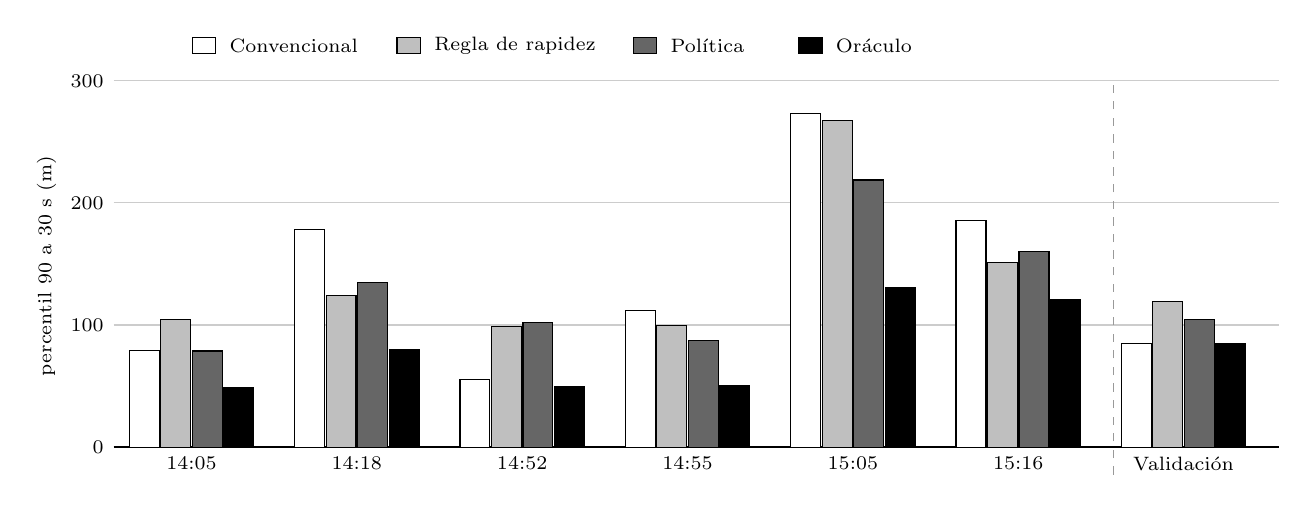
\begin{tikzpicture}[font=\scriptsize]
\def\ys{0.0155}
\foreach \v in {0,100,200,300} {
  \draw[black!20] (0,\v*\ys) -- (14.8,\v*\ys);
  \node[left] at (0,\v*\ys) {\v};
}
\draw[thick] (0,0) -- (14.8,0);
\node[rotate=90] at (-0.85,2.3) {percentil 90 a 30~s (m)};
\foreach \lab/\a/\b/\c/\d [count=\i] in {
  14:05/79.1/104.6/78.7/49.0,
  14:18/178.2/124.0/134.9/79.8,
  14:52/55.4/98.9/102.1/49.3,
  14:55/111.8/99.8/87.1/50.3,
  15:05/273.3/267.4/218.8/130.5,
  15:16/185.7/150.9/160.5/120.7,
  Validación/84.9/119.1/104.6/84.9} {
  \pgfmathsetmacro{\xo}{(\i-1)*2.1+0.2}
  \draw[fill=white] (\xo,0) rectangle ++(0.38,\a*\ys);
  \draw[fill=black!25] (\xo+0.4,0) rectangle ++(0.38,\b*\ys);
  \draw[fill=black!60] (\xo+0.8,0) rectangle ++(0.38,\c*\ys);
  \draw[fill=black] (\xo+1.2,0) rectangle ++(0.38,\d*\ys);
  \node[below] at (\xo+0.79,0) {\lab};
}
\draw[black!40, dashed] (12.7,-0.35) -- (12.7,4.6);
\begin{scope}[shift={(1.0,5.0)}]
  \draw[fill=white] (0,0) rectangle (0.3,0.2); \node[right] at (0.35,0.1) {Convencional};
  \draw[fill=black!25] (2.6,0) rectangle (2.9,0.2); \node[right] at (2.95,0.1) {Regla de rapidez};
  \draw[fill=black!60] (5.6,0) rectangle (5.9,0.2); \node[right] at (5.95,0.1) {Política};
  \draw[fill=black] (7.7,0) rectangle (8.0,0.2); \node[right] at (8.05,0.1) {Oráculo};
\end{scope}
\end{tikzpicture}
\caption[Percentil 90 del error a 30~s por sesión de prueba]{Percentil 90 del error al volver el GPS en los cortes de 30~s, por sesión de prueba, con la política de la primera iteración (media de tres semillas). La grabación de validación, a la derecha de la línea discontinua, pertenece a otro dominio. Fuente: elaboración propia.}
\label{fig:res-rl-sesiones}
\end{figure}

Por sesión (Fig.~\ref{fig:res-rl-sesiones}), la política mejora el percentil 90 en cuatro de las seis sesiones, lo iguala en la de las 14:05 y lo empeora en la de las 14:52, la más corta, con 9 cortes de 30~s; la regla empeora dos.
Los controles descartan un artefacto: una segunda corrida idéntica reprodujo los mismos números y la misma tabla final; con las mismas tablas pero con los estados barajados la captura cayó a 4 y 3~\%, y con acciones al azar en la misma proporción, a 8 y 7~\%; y un remuestreo por sesión dio intervalos del percentil 5 al 95 de 16 a 49~\% a 20~s y de 22 a 52~\% a 30~s.
En los cortes de 30~s que empiezan a menos de 3~m/s la política casi no cambia el resultado, mientras que por encima de 10~m/s descarta con frecuencia la rapidez de la cámara: rescata los cortes en que la escala se dispara, con un percentil 90 de mejora de 157~m, a cambio de empeorar otros, con un percentil 10 de $-61$~m.

La comparación más exigente es con un peso fijo menor para la cámara durante los cortes, elegido con las sesiones de entrenamiento: empata con la política en el percentil 90, pero empeora la mediana en 6 a 7~m, frente a 0,7 a 1,8~m de la política, porque baja el peso siempre, mientras que la política decide cuándo bajarlo.
El análisis de los cortes en que la política pierde más de 20~m mostró que su estado no distingue una cámara con la escala equivocada de un vehículo que acelera o frena, y que descartar la cámara equivale a suponer rapidez constante; esto motivó la segunda iteración, con pesos finitos intermedios.
En la grabación de validación no hubo margen a 30~s, ya que el oráculo coincide con el filtro convencional, y tanto la política como la regla empeoraron el percentil 90, aunque la mediana de la política quedó igual o mejor: la política no se traslada a un dominio con otra aplicación y otra cámara.
Durante los cortes, la política eligió $\lambda = 1$ en el 30 a 55~\% de las decisiones, $\lambda = 4$ en el 16 a 26~\% y el descarte en el 20 a 54~\%, y la tabla final visitó 187 de los 243 estados.

% Pendiente para discutir con la contraparte: Agregar los resultados de la segunda iteración y justificar la iteración que se adopta.

% ---------------------------------------------------------------------------
\subsection{Limitaciones de la solución}
\label{sec:res-limitaciones}
% CTX §4.25, §4.31 (punto 5), §4.33.

\begin{itemize}
\item \textbf{Referencia.} Las grabaciones propias carecen de una trayectoria de referencia de alta precisión.
El GPS del teléfono, con un error de varios metros, limita las comparaciones finas, aunque es pequeño frente a los errores de decenas de metros que se miden en los cortes.
\item \textbf{Latencia en la portátil.} La latencia en la computadora portátil empleada en campo es mucho mayor que en la computadora de escritorio: su percentil 95 fue de 167 a 189~ms conectada a la corriente y de 201 a 219~ms con batería, frente a 107~ms, porque su tiempo de procesamiento por cuadro es de dos a tres veces mayor.
\item \textbf{Escala de la cámara.} Varía con la escena y la rapidez, y se desploma por encima de 12~m/s; domina el error en los cortes de más de 20~s y con soluciones GPS escasas.
\item \textbf{Aprendizaje por refuerzo.} El aporte de la política es moderado y pierde confiabilidad fuera del dominio en que se entrenó.
Su limitación principal es que, durante una pérdida del GPS, el estado no distingue si la rapidez de la cámara es errónea o si el vehículo realmente aceleró o frenó.
En el segundo caso la política baja la confianza en la cámara cuando no debería, lo que equivale a suponer una rapidez constante y empeora ligeramente la estimación: la mediana del error al volver el GPS es de 0,7 a 1,8~m mayor que la del filtro convencional.
La política evaluada mejora los resultados frente al filtro convencional en los peores casos, pero esta limitación persiste.
\end{itemize}

%%% Local Variables:
%%% mode: latex
%%% TeX-master: "main"
%%% End:
